\documentclass{article}
\usepackage[utf8]{inputenc}
\usepackage{amsmath}
\usepackage{graphicx}

\title{SVM}
\author{Steven Wang}
\date{2017}

\begin{document}

\maketitle

\section{Intuition}
Assume there are 2 classes: - and + in a 2-dimensional space.
\\
We want to classify unknown samples into these 2 classes with SVM, by finding a hyperplane that best separates the 2 classes.
\\
In this case:
\\
\indent $\vec{u}$ is an unknown sample.
\\
\indent $\vec{w}$ is a vector perpendicular to the separation hyperplane.
\[
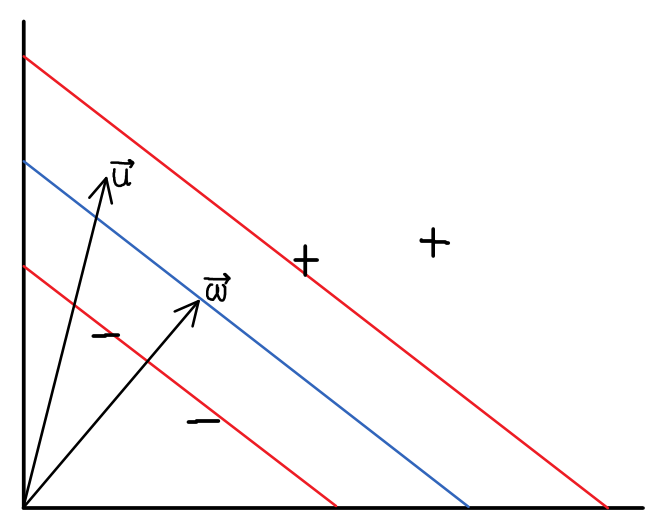
\includegraphics[scale=0.5]{fig_1}
\]
\\
Decision rule:
$$if\quad\vec{\omega}\cdot\vec{u}\geq c,\ then\quad\vec{u}\in+$$
$$(The\ projection\ of\ \vec{u}\ on\ \vec{w})$$
\\
More generally($c=-b$):
\\

\begin{equation} \label{eq:someequation}
    if\quad\vec{\omega}\cdot\vec{u}+b\geq0, \quad then \Rightarrow \vec{u}\in+
\end{equation}



\section{Question: What is $\vec{w}$ and $b$?}
Assume for known samples:
$$\vec{\omega}\cdot\vec{x}_+ + b\geq1$$
$$\vec{\omega}\cdot\vec{x}_- + b\leq-1$$
Now let's introduce a variable $y_i$ for mathematical convenience:
\\
$$y_i=\left\{\begin{array}{ll}
                +1 \qquad for + samples \\
                -1 \qquad for - samples
            \end{array}
        \right.$$
\\
$$\Rightarrow\left\{\begin{array}{cc}
    y_i(\vec{\omega}\cdot\vec{x}_+ + b)\geq1 \\
    y_i(\vec{\omega}\cdot\vec{x}_- + b)\geq1 \\
\end{array}
\right.$$
\\
$$\Rightarrow y_i(\vec{\omega}\cdot\vec{x}_i + b)-1\geq0$$
\\
Assume for $\vec{x}_i$ between(\&on) the 2 solid lines:
\begin{equation} \label{eq:someequation}
    \Rightarrow y_i(\vec{\omega}\cdot\vec{x}_i + b)-1=0
\end{equation}
\\
\[
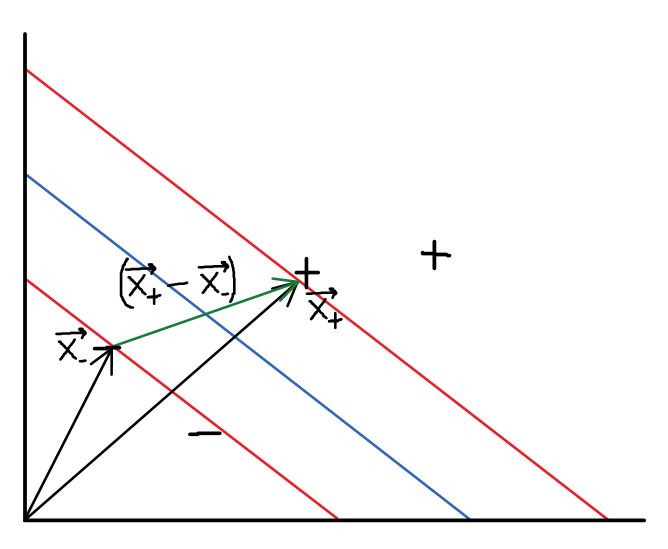
\includegraphics[scale=0.6]{fig_2}
\]
\\
$$\textbf{width}\ (between\ the\ red\ lines)=(\vec{x}_+-\vec{x}_-)\cdot\underbrace{\frac{\vec{\omega}}{||\vec{\omega}||}}_{\text{unit vector}}$$
$\frac{\vec{\omega}}{||\vec{\omega}||}$: This makes a unit vector that gives the direction perpendicular to separation hyperplane(a straight line here in this case).
\\
$$(2)\Rightarrow\left\{\begin{array}{cc}
        \vec{x}_+\vec{\omega}=1-b \\
        -\vec{x}_-\vec{\omega}=1+b \\
    \end{array}
\right.
$$
\begin{equation} \label{eq:someequation}
   \Rightarrow \textbf{width}=(1-b+1+b)\frac{1}{||\vec{\omega}||}=\frac{2}{||\vec{\omega}||}
\end{equation}


$\Rightarrow\quad$We want to max $\frac{1}{||\vec{\omega}||}$(maximize the margin of the separation hyperplane between the 2 classes).
$$\Rightarrow\quad min\{||\vec{\omega}||}\}\ \Rightarrow\quad min\{\frac{1}{2}}||\vec{\omega}||^2\}\quad(for\ mathematical\ convenience)$$

(How find extremum with constraints? $\Rightarrow Lagrange)$
$$L=\frac{1}{2}||\vec{\omega}||^2-\sum_i\alpha_i [y_i(\vec{\omega}\cdot\vec{x}_i+b)-1]$$

(How to take derivative of vectors? It has the same form of scalars.)
$$\frac{\partial L}{\partial\vec{\omega}}=\vec{\omega}-\sum_i\alpha_i y_i\vec{x}_i=0$$

\begin{equation} \label{eq:someequation}
    \Rightarrow\quad\vec{\omega}=\sum_i\underbrace{\alpha_i}_\text{(scalar)}\cdot\underbrace{y_i}_\text{(+1,-1)}\cdot\ \vec{x}_i
\end{equation}
It is proved to be a convex space, so no local extremum.
\\
\\
\\
\\
\subsection{*Important observation 1}
$\vec{\omega}$ is a linear sum of the sample vectors.
\\
\\
\\
\\
$$\frac{\partial L}{\partial b}=-\sum_i \alpha_i y_i=0 \Rightarrow \sum_i \alpha_i y_i=0$$
\\
Plug (4) into $L$:
$$
L=\frac{1}{2}(\sum_i\alpha_i y_i\vec{x}_i)(\sum_j\alpha_j y_i\vec{x}_j)-\sum_i\alpha_i y_i\vec{x}_i (\sum_j\alpha_j y_i\vec{x}_j)-\underbrace{\sum_i\alpha_i y_i}_\text{=0}\cdot\ b +\sum_i\alpha_i
$$
\begin{equation} \label{eq:someequation}
    L=\sum\alpha_i-\frac{1}{2}\sum_i\sum_j\alpha_i\alpha_j y_i y_j \underline{\vec{x}_i\vec{x}_j}
\end{equation}

\subsection{*Important observation 2}
Maximization depends only on the dot products of sample vectors.
\\
\\
\\
\\
Decision rule:
$$if\quad\sum_i\alpha_i y_i\vec{x}_i\cdot\vec{u}+b\geq0,\quad then\ +$$

\section{Linearly inseparable instances}
Apply transformation to sample vectors: $\phi(\vec{x})$
\\
(In this case, convert the samples from 2d to 3d space)
\\
\[
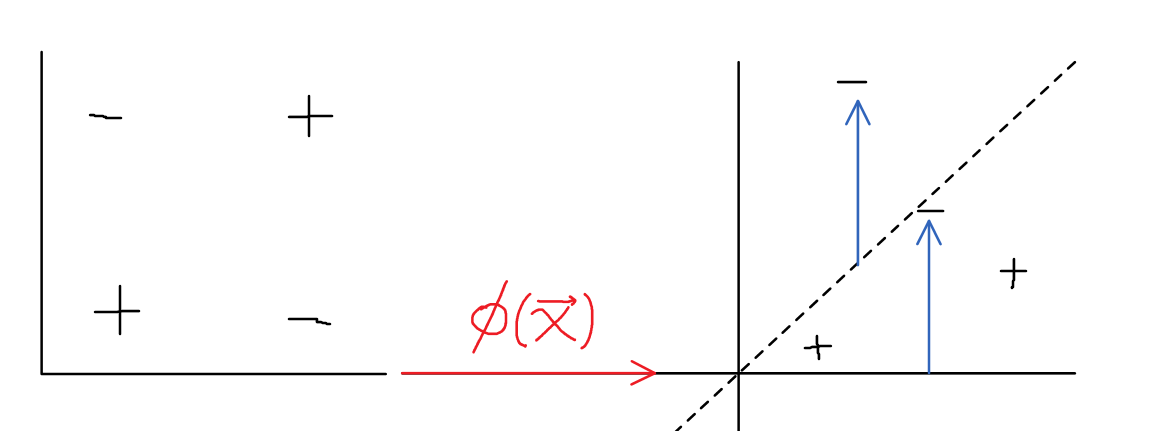
\includegraphics[scale=0.5]{fig_3}
\]
\\
Now the goal is:
$$max\{\phi(\vec{x}_i)\cdot\phi(\vec{x}_j)\}$$
And the decision rule contains:
$$\phi(\vec{x}_i)\cdot\phi(\vec{u}_j)$$
\\
If we can find kernel function:
$$K(\vec{x}_i\cdot\vec{x_j})=\phi(\vec{x}_i)\cdot\phi(\vec{x}_j)$$
Then we do not need the transformation $\phi$. Because $K$ provides the product of those 2 vectors in another space, I don't have to know the transformation $\phi$.

\section{Popular kernels}
\begin{itemize}
    \item linear kernel:
        $$(\vec{u}\vec{v}+1)^n$$
    \item radio basis function(rbf):
        $$e^{-\frac{||x_i-x_j||}{\sigma}}$$
\end{itemize}








\end{document}